\chapter{实验设计与分析}
\label{cha:expriment}

本文的目标是验证基于DTW距离度量的Shapelet并行算法在准确率不降的基础上,获得速度上的提升。
本章根据目标设计了一系列针对性的实验,验证Shapelet并行算法的速度问题,主要包括两部分:实验设计部分和实验结果分析部分。

\section{实验设计}

实验设计部分首先介绍了运行并行程序的实验环境和数据集,然后针对本文的目标设计了实验方案,最后介绍了我们针对本实验的评价指标。
%实验设计部分包括实验环境、实验数据、实验方案和评价方法。
\subsection{实验环境}
首先介绍本文的实验环境,实验环境分为以下几个部分:

1.其中硬件环境如表~\ref{tab:computerversion}和表~\ref{tab:gpuversion}。

2.其中软件环境如表~\ref{tab:software}。

3.开发和调试主要使用$cuda$自带的$cuda-gdb$,$gcc/g++$和$nvcc$的优化等级都为$O3$。

\begin{table}[htb]
	\centering
	\begin{minipage}{0.5\textwidth}
		\centering
		\caption{硬件环境-主机参数}
		\label{tab:computerversion}
		\begin{tabular}{p{4cm}p{2cm}}
			\toprule[1.5pt]
			硬件描述 & 版本或大小 \\
			\midrule[1pt]
			CPU & i7-7700 \\
			内存 & 16G  \\
			主频 & 3.6GHz  \\
			\bottomrule[1.5pt]
		\end{tabular}
	\end{minipage}%
\end{table}

\begin{table}[htb]
	\centering
	\begin{minipage}{0.5\textwidth}
	\centering
	\caption{硬件环境-图形处理器参数}
	\label{tab:gpuversion}
		\begin{tabular}{p{4cm}p{2cm}}
			\toprule[1.5pt]
			硬件描述 & 版本或大小 \\
			\midrule[1pt]
			GPU型号 & GTX-1080 \\
			全局内存 & 8G \\
			流处理器 & 20*128 \\
			共享内存(每个Block) & 48K \\
			寄存器(每个Block) & 64K \\
			\bottomrule[1.5pt]
		\end{tabular}
	\end{minipage}
\end{table}

\begin{table}[htb]
	\centering
	\begin{minipage}{0.5\textwidth}
		\caption{软件环境}
		\label{tab:software}
		\begin{tabular}{p{3cm}p{3cm}}
			\toprule[1.5pt]
			{\heiti 软件} & {\heiti 版本} \\\midrule[1pt]
			操作系统 & ubuntu 16.04 \\
			GUN Make & 4.1 \\
			gcc/g++ & 5.4.0 \\
			Cuda & 8.0 \\
			计算能力 & 6.1 \\
			NVCC & 8.0.61 \\
			\bottomrule[1.5pt]
		\end{tabular}
	\end{minipage}
\end{table}

\subsection{实验数据}
为了方便和优化工作及并行算法比较,本文使用的UCR时间序列分类~\cite{UCRArchive}。本实验选取数据集中的二分类数据作为本实验的实验数据,本文只考虑二分类问题,延展到多分类问题不在本文介绍。表~\ref{tab:dataset}是关于数据的类标、大小、序列长度等信息的介绍。
%把数据叙述一下。
%下面这一部分可以用于DataSet
%
%工业数据时间序列的重要性。
%时间序列分类(TSC)问题与传统的分类问题是不同的,因为属性是有序的。 事实上,顺序是否与时间无关,实际上是无关紧要的。 重要的特征是可能存在依赖于排序的歧视性特征。 UCR时间序列分类和聚类库[21]的引入使提出时间序列分类算法的出版物数量迅速增长。 在2015年夏天之前,超过1,200人下载了UCR档案,并且它已被引用数百次。 该知识库有助于提高新TSC算法评估的质量。 大多数实验涉及评估超过四十个数据集,通常具有正确的重要性测试,大多数作者发布源代码。 这种评估和再现性的程度通常比机器学习和数据挖掘研究的大多数领域更好

\begin{table}[htbp]
	\centering
	\begin{minipage}{0.9\textwidth}
		\caption{实验数据集}
		\label{tab:dataset}
		\begin{tabular}{p{3cm}p{2cm}p{2cm}p{2cm}p{2.5cm}}
			\toprule[1.5pt]
			{\heiti 数据集名称} &{\heiti 类标 } & {\heiti 训练集大小} &{\heiti 测试集大小} &{\heiti 时间序列长度}\\\midrule[1pt]
			ECGFiveDays &2(1,-1) &23 &861 &136\\
			Coffee  &2(0,1) &28 &28 &286 \\
			Gun-Point    &2(1,2)&50&150&150\\
			WormsTwoClass&2(1,2)&77&181&900\\
			ECG200          &2(1,-1)&100&100&96\\
			Ham          &2(1,2)&109&105&431\\
			Yoga         &2(1,2)&300&3000&426\\
			Strawberry   &2(1,8)&370&613&235\\
			Wafer        &2(1,-1)&1000&6174&152\\
			FordA &2(1,-1) &1320 &3601 &500 \\
			\bottomrule[1.5pt]
		\end{tabular}
	\end{minipage}
\end{table}

\subsection{实验方案设计}
第三章介绍了并行算法的总体方案以及距离度量选择,因此需要考虑参数$w$对于性能指标的影响,并将本实验和已有优化工作进行指标比较。第四章介绍三个模块的并行算法及优化方法,因此需要对优化方法对对应模块的作用进行评估。基于以上考虑,需要对以下几个方面进行评估:

%1.算法的准确率和总体执行时间,以及和已有算法进行比较;
1.$w$发生变化时,对于算法评价指标的影响;

2.距离计算阶段执行时间与$N,L$变化的关系;

3.$w=0$距离计算阶段执行时间与$N,L$变化的关系;

4.比较最佳分割点计算阶段原始算法、启发式计算最佳分割点算法的指标比较。

5.计算最佳分割点阶段执行时间与$N,L$变化的关系;

6.对于一些重要优化方法,需要指出优化方法对于执行时间的优化效果。
\subsection{评价方法}

本文的主要目的是在保证准确率不降或者微降的基础上尽可能提高执行效率,所以这里只有两个评价指标:准确率和时间。

准确率是将样本的预测$pred_j,j=1,2,\cdots,N$和类标$y_j,j=1,2,\cdots,N$进行统计,可以表示为$Aurracy=\sum_{h=1}^{N}\textstyle 1\left\lbrace pred_j=y_j\right\rbrace/N$,其中$\textstyle 1\{\cdot\}$为示性函数,表达式为$\textstyle 1\{ \text{值为真的表达式} \textstyle \}=1$。

执行时间的计算和CPU统计执行时间略有不同,GPU统计时间必须等所有Block运行完毕之后才能进行统计时间,这里使用CUDA的$nvprof$或者$Events$来统计执行时间~\cite{nvidia2015c}。

在实际统计执行时间时,没有将申请全局内存和数据集拷入的时间计算在内。因为申请内存和拷贝的时间比较固定,大约$200\sim 600ms$之间,对于大数据集没有影响,对于小数据集影响很大,为了方便比较,没有将这些时间计入执行时间。

\section{实验结果分析}

%首先对于基于DTW距离度量的Shapelet算法的准确率和已有Shapelet算法、深度学习的准确进行比较。表~\ref{tab:accuracy}是不同数据集下,深度学习算法和本算法就准确率方面进行比较。

%\begin{table}[htbp]
%	\centering
%	\begin{minipage}{0.7\textwidth}
%		\caption{各算法在不同的数据集的准确率表现}
%		\label{tab:accuracy}
%		\begin{tabular}{p{5cm}p{2cm}p{2cm}}
%			\toprule[1.5pt]
%			{\heiti 数据集} &{\heiti 深度学习 } & {\heiti 本算法} 
%			\\\midrule[1pt]
%			Gun\_Point    & - & 0.8495 \\
%			wafer & - & 0.953215 \\
%			ECG200 & - & 0.86 \\
%			ECGFiveDays & - & 0.966039 \\
%			Coffe & - & 0.801429 \\
%			Ham & - & 0.628571 \\
%			Strawberry & - & 0.794454 \\
%			Yoga & - & 0.646167 \\
%			FordA & - & 0.788 \\
%			FordB & - & 0.802 \\
%			\bottomrule[1.5pt]
%		\end{tabular}
%		\footnotesize 注 -:{\color{red}{数据后补}}
%	\end{minipage}
%\end{table}

实验分析部分首先对于整体执行过程的指标进行比较,然后分别对w>0距离计算阶段,w=0距离计算阶段,最佳分割点计算阶段的优化方法的效果进行比较。
%本文的主要目的是保证准确率的基础上对于基于DTW距离度量的Shapelet算法进行加速,后文主要看算法的执行效率,主要从总体执行时间、距离计算阶段时间分析、最佳分割点计算时间分析三个方面进行介绍。

\subsection{总体指标比较}
\label{cha:chap05:Analysis:Overall}

表~\ref{tab:CompareWithOthers}是\textbf{并行执行时间和CPU执行时间以及已有优化执行时间的比较}。表~\ref{tab:CompareWithOthers}中实验使用的距离度量为$Dist(A,B)$。
%其中部分数据集CPU时间是根据一个时间序列$T_1$中的候选序列$SubSet(T_1)$的时间时间的$N$计算的。
%比较数据中部分也是换算而来,较大数据文中只计算了候选序列长度$|S|\%10==0$的情况。

\begin{table}[htbp]
	\centering
	\begin{minipage}{0.9\textwidth}
		\caption{整体执行时间和已有工作的比较}
		\label{tab:CompareWithOthers}
		\begin{tabular}{p{2cm}p{1cm}p{1cm}p{1.8cm}p{1.8cm}p{1.8cm}p{1.5cm}}
			\toprule[1.5pt]
			{\heiti 数据集} & {\heiti N } &{\heiti L } &{\heiti CPU(s) } &{\heiti 文献~\cite{renard2015random}(s) } &{\heiti 文献~\cite{chang2012efficient}(s) } &{\heiti 我们(s) }
			\\\midrule[1pt]
			Coffee & 28 & 286 & 829.3 & 8.1$^-$ &  3 & 0.372 \\
			GUN\_POINT & 50 & 150 & 143.6 & 9.2$^-$ & 1.2 & 0.172 \\
			ECG200 & 100 & 96 & 151.5 & 7.6$^-$ & 1.6 & 0.155 \\
			%Lighting2 & * & * & - & 17 & *\\
			wafer & 1000 & 152 & 15471.7$^+$ & NA$^*$ & 546$^{**}$ & 25.7 \\
			FordB & 810 & 500 & 3013203$^+$ & NA$^*$ & NA$^*$ & 816 \\
			FordA & 1320 & 500 & 8002140$^+$ & NA$^*$ & NA$^*$ &  2398\\
			\bottomrule[1.5pt]
		\end{tabular}
	    \footnotesize -:使用文献~\cite{renard2015random}中采样概率为1\%的数据 \\
		+:使用$SubSet(T_1)$候选集的执行时间$*N$作为CPU执行时间 \\
		*:无对比数据 \\
		**:通过原始数据$*10$获得,因为文献使用的是候选序列子集\\
	\end{minipage}
\end{table}

从表~\ref{tab:CompareWithOthers}可以看出,基于DTW距离度量的Shapelet并行方案相比已有的加速算法有很大的提高,其中相比原始CPU算法提高834到3692倍,平均1945倍;相比Random-Shapelet~\cite{renard2015random}提高21倍到51倍之间,平均41倍;相比已有GPU并行算法提高3倍到21倍,平均13倍。已有优化工作因为各种原因对于UCR较大数据集没有涉及,而本文并行算法对于UCR~\cite{UCRArchive}中最大的数据集也进行了实验。

下面分析\textbf{$w$的参数对于准确率/执行时间的影响},$DTW(A,B,w)$距离度量中$w$的参数变化会导致准确率/执行时间的变化,表~\ref{tab:metricdpw}中表示不同的数据集中,随着$w$的变化,准确率/整体执行时间(秒)的变化,其中,$w=0$处使用的是$Euclid(A,B)$的距离度量,表格中是$w=0$距离计算的执行时间。
\begin{table}[htbp]
	\centering
	\begin{minipage}{\textwidth}
		\caption{评价指标随$w$的变化}
		\label{tab:metricdpw}
		\begin{tabular}{p{1.8cm}p{1.8cm}p{1.8cm}p{1.8cm}p{1.8cm}p{1.8cm}p{1.8cm}}
			\toprule[1.5pt]
			{\heiti 数据集} &{\heiti $w=0$($s/\sim$) } &{\heiti $w=1$($s/\sim$) } &{\heiti $w=2$($s/\sim$) } &{\heiti $w=3$($s/\sim$) } &{\heiti $w=4$($s/\sim$) } &{\heiti $w=5$($s/\sim$) }
			\\\midrule[1pt]
			Gun-Point    & 0.8450/0.205 & 0.8530/0.837 & 0.8620/1.098 & 0.8490/1.343 & 0.8230/1.576 & 0.8170/1.781 \\
			wafer & 0.9528/25.71 & 0.9530/121.2 & 0.9531/197.3 & 0.9529/278.3 & 0.9531/356.7 & 0.9532/432.7 \\
			ECG200 & 0.8000/0.592 & 0.8000/0.951 & 0.8600/1.249 & 0.7900/1.489 & 0.8100/1.758 & 0.8100/2.000 \\
			ECGFiveDays &  0.9660/0.136 & 0.9421/0.235 & 0.8126/0.347 & 0.5797/0.409 & 0.5838/0.528 & 0.6000/0.607 \\
			Coffee & 0.8014/0.882 & 0.7346/1.370 & 0.6846/1.905 &0.6896/2.403 & 0.6843/2.890 & 0.7321/3.417 \\
			Ham & 0.6286/22.16 & 0.5000/45.57 & 0.4571/74.70 & 0.5714/102.7 & 0.5714/130.2 & 0.5047/159.7 \\
			Straw & 0.7944/30.67 & 0.6949/72.35 & 0.6199/116.6 & 0.5383/160.6 & 0.5465/209.3 & 0.4665/255.1 \\
			Yoga & 0.6437/138.9 & 0.6397/319.4 & 0.6462/521.3 & 0.6442/725.8 & 0.6387/920.8 & 0.6427/1124 \\
			%			FordA & 0.788/2398 & 0.758/9654 & - & - & - & - \\
			%			FordB & - & - & - & - & - & - \\
			\bottomrule[1.5pt]
		\end{tabular}
		%\footnotesize 注-:{\color{red}{数据后补}}
	\end{minipage}
\end{table}

从表~\ref{tab:metricdpw}可以看出随着$w$在$ 0 \to |S|$变化时,执行时间呈线性变化,而大部分数据的准确率承呈先升后降,如GUN\_POINT数据,从$w=0$的0.8450到$w=2$处取得最大值0.862,之后准确率逐渐下降。有的数据准确率的最大值就在$w=0$处,如ECGFiveDay。有两个原因可以解释这件事,一方面,一些时间序列存在固定的模式匹配,不具有伸缩性质,而这些模式就是进行时间序列分类的关键;另一方面,$DTW(A,B,w)$具有对于时间序列平移、伸缩来进行时间序列之间的相似性匹配,但是Shapelet算法中候选序列$S$和时间序列$T_j$是以滑动窗口的方式进行距离比较$Dist(S,T_{j,s}^{|S|}),s=1,2,\cdots,L-|S|+1$也具有进行时间序列平移匹配的性质,这样使得$DTW(A,B,w)$平移性质没有得到发挥。

这里我们可以得到一个结论:采用$DTW(A,B,w)$距离度量保证分类准确率大于等于$Dist(A,B)$距离度量的准确率。

\textbf{并行方案中不同阶段的执行时间及占比},并行方案分为三个阶段:距离计算阶段、最佳分割点计算阶段、候选序列筛选阶段。如表~\ref{tab:OverviewTime}分别是各个数据集在三个阶段的执行时间及占比。其中,由于数据太多的原因,表~\ref{tab:OverviewTime}中对于每个数据集只列举了部分$w$下的各阶段执行时间及占比,表中的其他是指除了距离计算阶段和最佳分割点计算阶段之外的其他阶段(包含候选序列筛选计算在内)。

\begin{table}[htbp]
	\centering
	\begin{minipage}{0.9\textwidth}
		\caption{不同阶段执行时间在不同数据集下的表现}
		\label{tab:OverviewTime}
		\begin{tabular}{p{2cm}p{1cm}p{2cm}p{2cm}p{2.5cm}p{2cm}}
			\toprule[1.5pt]
			{\heiti 数据集} &{\heiti $w$ } &{\heiti 总时间(s) } &{\heiti 距离计算(s) } &{\heiti 最佳分割点(s) } &{\heiti 其他(s) }
			\\\midrule[1pt]
			GUN\_POINT & 2 & 1.099 & 1.039(0.946) & 0.044(0.04) & 0.015(0.014)\\
			wafer & 0 & 25.717 & 15.362(0.597) & 10.335(0.402) & 0.02(0.001)\\
			ECG & 4 & 1.758 & 1.654(0.941) & 0.084(0.048) & 0.02(0.011)\\
			ECGFiveDays & 2 & 0.347 & 0.326(0.938) & 0.006(0.016) & 0.016(0.045)\\
			Coffee & 4 & 2.89 & 2.845(0.984) & 0.033(0.011) & 0.013(0.004)\\
			Ham & 3 & 102.763 & 101.009(0.983) & 1.73(0.017) & 0.024(0.000)\\
			Strawberry & 1 & 72.351 & 68.704(0.95) & 3.62(0.050) & 0.027(0.000)\\
			Yoga & 0 & 138.949 & 130.438(0.939) & 8.482(0.061) & 0.029(0.000)\\
			\bottomrule[1.5pt]
		\end{tabular}
	\end{minipage}
\end{table}

\begin{figure}[H] % use float package if you want it here
	\centering
	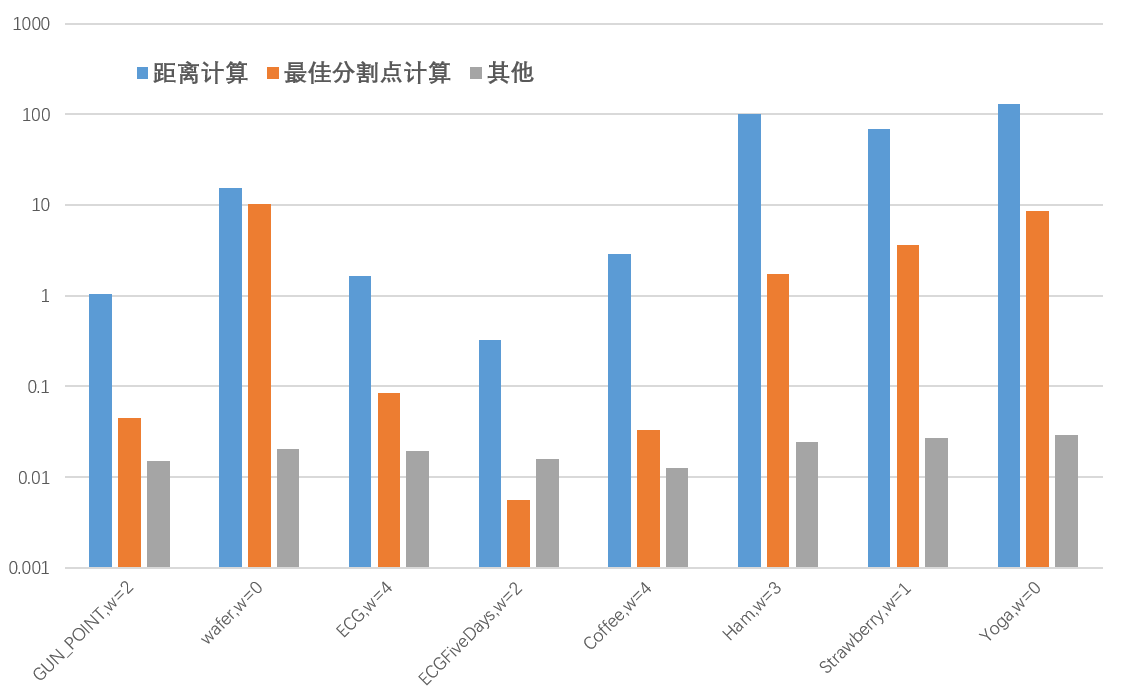
\includegraphics[height=8.2cm]{3PhaseTimewithData.png}
	\caption{不同阶段执行时间在不同数据集下的表现}
	\label{fig:3PhaseTimewithData}
\end{figure}

图~\ref{fig:3PhaseTimewithData}是表~\ref{tab:OverviewTime}的图示效果,其中纵轴执行时间采用基数为10的对数刻度。从表~\ref{tab:OverviewTime}和~\ref{fig:3PhaseTimewithData}可以看出距离计算占比最大,其次是最佳分割点计算阶段,包含候选序列筛选阶段在内的其他阶段占比不超过1\%。而且$N$很大,$L$比较小的情况下,距离计算阶段和最佳分割点计算阶段的执行时间比较接近。
%时间占比主要和$L$有关,$L$越大,距离计算阶段占比越大。

\textbf{各阶段执行时间与$w$的关系},表~\ref{tab:Timewithw}是使用数据集wafer在不同的$w$计算下各阶段执行时间。使用相同数据集的情况下随着$w$的变化,最佳分割点计算阶段和其他阶段的执行时间基本不变。而距离计算阶段执行时间随着$w$增大不断变化,从图~\ref{fig:Wafer3PhaseTimewithW}可以基本呈线性关系,执行时间占比不断增高。

\begin{table}[htbp]
	\centering
	\begin{minipage}{0.9\textwidth}
		\caption{各阶段执行时间与$w$的关系(wafer数据集)}
		\label{tab:Timewithw}
		\begin{tabular}{p{2cm}p{2cm}p{2cm}p{3cm}p{2cm}}
			\toprule[1.5pt]
			 {\heiti $w$ } &{\heiti 总时间(s) } &{\heiti 距离计算(s) } &{\heiti 最佳分割点(s) } &{\heiti 其他(s) }
			\\\midrule[1pt]			
			$w=0$ & 25.7168 & 15.3619 & 10.3345 & 0.0204\\
			$w=1$ & 121.239 & 110.860 & 10.3572 & 0.0218\\
			$w=2$ & 197.362 & 186.967 & 10.3738 & 0.0212\\
			$w=3$ & 278.350 & 267.948 & 10.3812 & 0.0208\\
			$w=4$ & 356.729 & 346.335 & 10.3731 & 0.0209\\
			$w=5$ & 432.687 & 422.306 & 10.3594 & 0.0216\\
			\bottomrule[1.5pt]
		\end{tabular}
	\end{minipage}
\end{table}

\begin{figure}[H] % use float package if you want it here
	\centering
	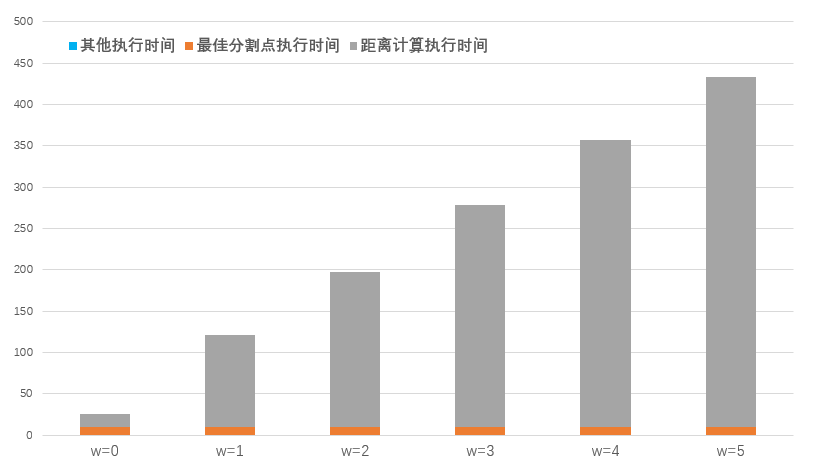
\includegraphics[height=7.2cm]{Wafer3PhaseTimewithW.png}
	\caption{各阶段执行时间与$w$的关系(wafer数据集)}
	\label{fig:Wafer3PhaseTimewithW}
\end{figure}

\subsection{w>0距离计算阶段时间分析}

在章节~\ref{cha:chap04:myalg:DTW:trick}中,w>0距离计算阶段主要使用了Coalesced合并内存访问和Bank-Conflict存储体冲突两个Cuda优化技术和算法结合,本章节主要看一下这些优化技术对于距离计算阶段执行时间的影响。%本章节中的所有时间都是距离计算阶段执行时间而不是总体执行时间。

\textbf{用合并内存访问对于总体执行时间的影响},表~\ref{tab:TimeCoalesced}表示关于在距离计算阶段是否使用Coalesced对于总体执行时间的影响。%因为Coalesced需要距离计算阶段和最佳分割点计算阶段配合执行,所以需要统计整体执行时间。%又因为Coalesced的主要策略都是在距离计算阶段进行的,因此将Coalesced对于执行时间的影响放在本章节。

\begin{table}[htbp]
	\centering
	\begin{minipage}{0.85\textwidth}
		\caption{是否Coalesced的总体执行时间在不同数据集下的表现}
		\label{tab:TimeCoalesced}
		\begin{tabular}{p{3cm}p{1cm}p{2cm}p{2.5cm}p{2cm}}
			\toprule[1.5pt]
			{\heiti 数据集 }& {\heiti $w$ } &{\heiti Coalesced(ms) } &{\heiti No~Coalesced (ms) } &{\heiti 时间差 百分比 }
			\\\midrule[1pt]			
				GUN\_POINT & w=4 & 1575.89 & 1716.1 & 0.082\\
				GUN\_POINT & w=1 & 837.496 & 904.68 & 0.074\\
				ECGFiveDays & w=4 & 528.163 & 586.40 & 0.099\\
				Coffee & w=5 & 3417.50 & 3654.5 & 0.065\\
				Coffee & w=0 & 882.365 & 1112.9 & 0.207\\
				Ham & w=3 & 102763 & 104029 & 0.012\\
			\bottomrule[1.5pt]
		\end{tabular}
	\end{minipage}
\end{table}

\begin{figure}[H] % use float package if you want it here
	\centering
	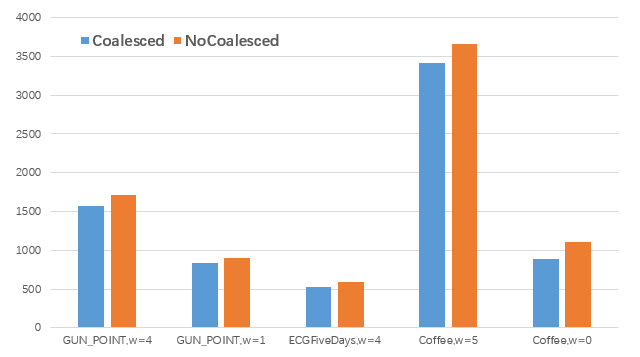
\includegraphics[height=7.2cm]{CoalescedDTW.png}
	\caption{是否Coalesced的总体执行时间在不同数据集下的表现}
	\label{fig:CoalescedDTW}
\end{figure}

从表~\ref{tab:TimeCoalesced}和图~\ref{fig:CoalescedDTW}可以看出,使用合并内存访问比普通的多线程连续地址访问效率要高,执行时间要少$1\sim 20\%$之间。%而且使用Coalesced合并内存访问会不会出现同一个连续的128B空间需要被两个SM缓存的情况。

\textbf{存储体冲突对于执行时间的影响},表~\ref{tab:BankConflictTimeWithW}是对于w>0距离计算阶段是否存在存储体冲突(Bank-Conflict)的距离计算阶段在不同$w$的执行时间进行比较。其中,$w=0$下的执行时间是基于$DTW(A,B,w=0)$距离计算的,$stride$是半个Warp内连续两个线程执行相同的操作的地址间隔。发现存在存储体冲突的执行时间普遍比没有存储体冲突执行时间长,而且在$stride=8,14,16$处尤为明显。存在存储体冲突的距离计算中:当$w=2$时,两个线程之间的stride为$2*(w+2)=8$,整个“8-way Bank Conflict”即每8线程访问同一个Bank的不同地址;而$w=5,stride=14$处出现的时“2-way Bank Conflict”,但是由于$w=5$每个线程访问Bank次数比较多所以导致使时间差异比较大;当$w=6$时,连续两个线程间隔$2*(w+2)=16$,半个Warp中的所有线程访问相同的Block中不同的地址出现“16-way Bank-Conflict”,这个在存储体冲突访问中是最严重的,所以时间差异最大。图~\ref{fig:BankConflictColumnar}是两者执行时间随$w$的变化,最初$w>0$距离计算阶段存在存储体冲突的问题也是通过此图$w=6$的尖峰异常发现的。

\begin{table}[htbp]
	\centering
	\begin{minipage}{0.9\textwidth}
		\caption{是否存在存储体冲突距离计算阶段执行时间与$w$的关系(wafer数据集)}
		\label{tab:BankConflictTimeWithW}
		\begin{tabular}{p{2cm}p{1cm}p{2cm}p{2cm}p{2cm}p{2cm}}
			\toprule[1.5pt]
			{\heiti $w$ } &{\heiti $stride$ } &{\heiti Bank-Conflict(s) } &{\heiti No-Bank-Conflict(s) } &{\heiti 差(s) } &{\heiti 访问Bank次数 }
			\\\midrule[1pt]							
				$w=0$ & 4 & 43.4377 & 43.5549 & 0.1172 & 6.5e5 \\
				$w=1$ & 6 & 110.860 & 122.403 & 11.543 & 9.7e5 \\
				$w=2$ & 8 & 186.967 & 205.580 & 18.613 & 1.2e6 \\
				$w=3$ & 10 & 267.948 & 274.802 & 6.8540 & 1.6e6 \\
				$w=4$ & 12 & 346.335 & 347.883 & 1.5480 & 1.9e6 \\
				$w=5$ & 14 & 422.306 & 445.596 & 23.290 & 2.3e6 \\
				$w=6$ & 16 & 496.314 & 629.338 & 133.02 & 2.6e6 \\
				$w=7$ & 18 & 571.834 & 595.752 & 23.918 & 2.9e6 \\
			\bottomrule[1.5pt]
		\end{tabular}
	\end{minipage}
\end{table}

\begin{figure}[H] % use float package if you want it here
		\centering
		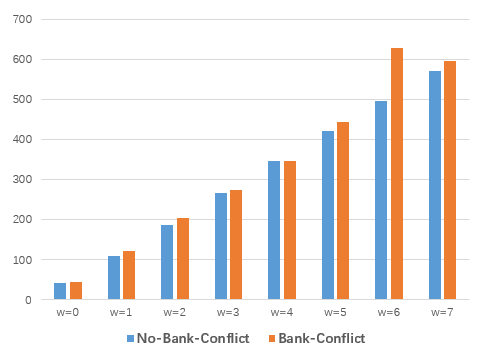
\includegraphics[height=8.2cm]{BankConflictColumnar.png}
		\caption{是否存在存储体冲突距离计算阶段执行时间与$w$的关系(wafer数据集)}
		\label{fig:BankConflictColumnar}
\end{figure}


\subsection{w=0距离计算阶段时间分析}

在距离计算和最佳分割点计算之间有增加了一个转置过程,因此使用总的执行时间来进行比较。

\begin{table}[htbp]
	\centering
	\begin{minipage}{0.72\textwidth}
		\caption{转置对于$w=0$时并行总体计算总体执行时间的影响}
		\label{tab:transpose}
		\begin{tabular}{p{3cm}p{3cm}p{3cm}}
			\toprule[1.5pt]
			{\heiti 数据集 } &{\heiti 实现转置(ms) } &{\heiti 直接存储(ms) }
			\\\midrule[1pt]							
			GUN\_POINT & 172.816 & 205.170 \\
			ECG200 & 155.726 & 172.474\\
			ECGFiveDays & 17.8826 & 20.9651\\
			Coffee & 127.688 & 152.241\\
			Strawberry & 11559.5 & 12946.3\\
			wafer & 25716.8 & 39719.9 \\
			\bottomrule[1.5pt]
		\end{tabular}
	\end{minipage}
\end{table}

从表~\ref{tab:transpose}可以看出,使用矩阵转置的方法比直接存储执行时间更短,说明转置过程使距离计算和最佳分割点计算访问内存都可以通过合并内存访问进行,使得延时等待的时间大大减少,而且转置过程本身也是全局内存访问的经典应用,访存等待时间较短,总的来说转置过程使w=0时的并行计算效率提升很多。

\subsection{最佳分割点计算时间分析}

\begin{table}[htbp]
	\centering
	\begin{minipage}{0.95\textwidth}
		\caption{计算最佳分割点的启发式算法和传统算法的比较}
		\label{tab:ShuffleWork}
		\begin{tabular}{p{2cm}p{1cm}p{1cm}p{2cm}p{2cm}p{1.5cm}p{1.5cm}}
			%			\hline
			\toprule[1.5pt]
			\multirow{2}{*}{{\heiti 数据集}} 
			& \multirow{2}{*}{{\heiti N}} 
			& \multirow{2}{*}{{\heiti L}}
			& \multicolumn{2}{c}{{\heiti 原始最佳分割点算法 }} & \multicolumn{2}{c}{{\heiti  启发式 }}  \\ \cmidrule[1.2pt]{4-7}
			&&& 时间(ms)         & 准确率         & 时间(ms)         & 准确率      
			\\\midrule[1pt]
			GUN\_POINT & 50 & 150 & 275.370 & 0.849 & 99.2050 & 0.845\\
			ECG200 &100 &96 & 363.013 & 0.800 & 135.543 & 0.800\\
			ECGFiveDays & 23 & 136 & 124.928 & 0.962 & 5.94600 & 0.963\\
			Coffee & 28 &286 & 525.071 & 0.806 & 77.6015 & 0.811\\
			Strawberry &370  & 235& 8284.36 & 0.801 & 3663.46 & 0.794\\
			Yoga & 300 & 426 & 24883.4 & 0.648 & 8406.19 & 0.644\\
			Ham &109 &431& 4668.29 & 0.614 & 1744.19 & 0.629\\
			wafer &1000 &152 & NA$^*$ & 0.953 & 10334.5 & 0.953\\
			\bottomrule[1.5pt]
		\end{tabular}\\
		\footnotesize *:需要资源太多,图形处理器不能执行 \\
		%注-:{\color{red}{数据后补}}
	\end{minipage}
\end{table}

本章节针对章节~\ref{cha:chap04:myalg:infogain}提出的启发式计算最佳分割点以及Shuffle进行验证。为了获取启发式算法和原始算法的评价指标关系以及使用Shuffle对于指标的影响,需要对于原始最佳分割点算法、启发式计算最佳分割点进行多个数据集下准确率和执行时间指标的评价。表~\ref{tab:ShuffleWork}是对于两种算法在不同数据集下的时间/准确率表现,其中时间只是最佳分割点计算阶段的执行时间。

从表~\ref{tab:ShuffleWork}可以看出启发式算法可以在准确率不降或者微降的前提下大幅度提高执行效率,平均提速2倍左右(仅对于最佳分割点阶段执行时间)。

\section{本章小结}

本章对于基于DTW距离度量的Shapelet并行算法在多个时间序列集上进行了验证,首先进行了实验环境、实验环境、实验数据、评价指标的介绍,然后在准确率方面和深度学习进行了比较;在执行时间方面和已有的加速算法进行比较;最后对于文中使用的优化技术分别进行了验证,肯定了优化技术对于性能的提高,这有优化技术包括距离计算阶段的合并内存访问和存储体冲突,$w=0$距离计算阶段的矩阵转置,计算最佳分割点阶段的启发式算法。
